\iffalse
\subsection{Нейронные сети для обработки текста}
В 2013-2014 годах нейросети (в первую очередь - рекуррентные, сверточные и рекурсивные) стали активно использоваться для обработки текста.  Наиболее широко в то время использовались три основных типа нейронных сетей: рекуррентные нейронные сети, сверточные нейронные сети и рекурсивные нейронные сети. Они будут подробнее описаны ниже, в разделах \ref{ch:nn:rnn}, \ref{ch:nn:cnn} и \ref{ch:nn:rcnn}.

\subsubsection{Рекуррентные нейронные сети}\label{ch:nn:rnn}
Рекуррентные нейронные сети (RNN) лучше всего подходят для работы с динамическими входными последовательностями, из которых и состоит естественный язык.  Первые рекурсивные сети были предложены Элманом в 1990 году~\cite{elman_1990}, но в 1997 году на их место пришли предложенные Шмитхубером сети долговременной памяти(LSTM) \cite{hochreiter_1997}, которые оказались более устойчивыми к проблеме исчезания/взрыва градиентов. В 2013 году Илья Суцкевер предложил в своей диссертации новый, более эффективный метод обучения LSTM \cite{suskever_2013}. Также в 2013 году Грэйвсом были предложены двунаправленные LSTM~\cite{graves_2013}, которые обычно используется для работы с левым и правым контекстом. Визуализацию ячейки LSTM можно увидеть на рисунке \ref{fig:Neuro3-LSTM}.  


\begin{figure}[ht]
  \centerfloat{
    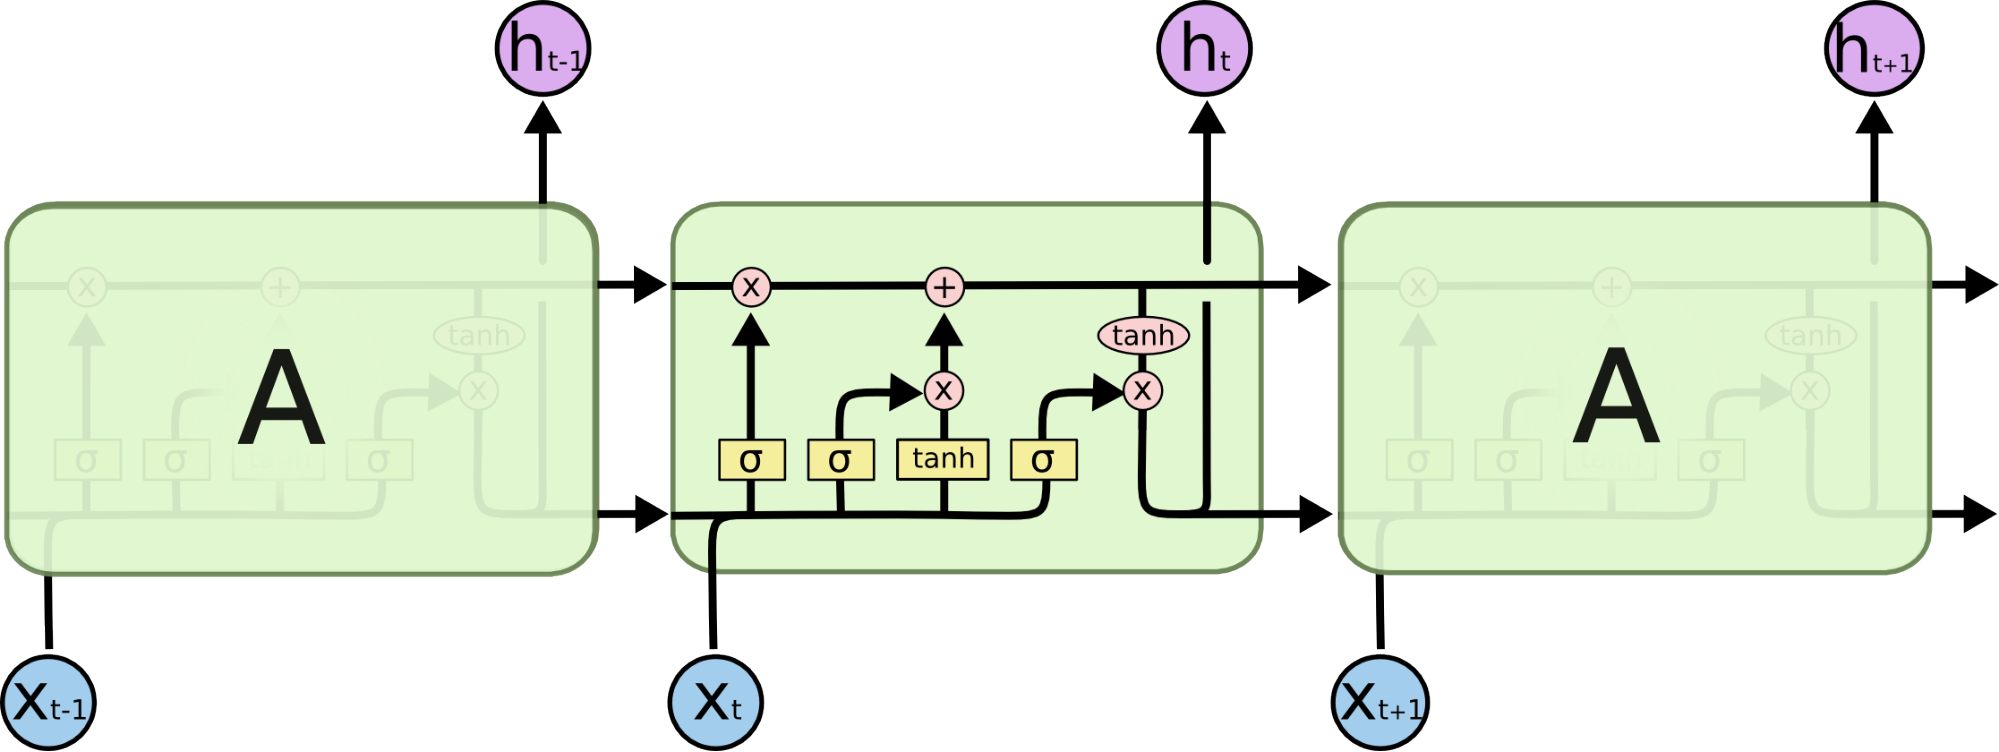
\includegraphics[width=\textwidth]{images/Neuro3-LSTM_.png}
  }
  \caption{Визуализация ячейки LSTM}\label{fig:Neuro3-LSTM}
\end{figure}


\subsubsection{Сверточные нейронные сети}\label{ch:nn:cnn}
Сверточные нейронные сети работают на основе операции свертки в двух измерениях, в 2014 году \cite{kalchbrenner_2014} они начали применяться в области обработки естественного языка. Преимуществом сверточных нейронных сетей, по сравнению с рекуррентными, является их распараллеливаемость. На рисунке \ref{fig:Neuro4-CNN} показан пример сверточной нейронной сети, используемой в обработке текста.


\begin{figure}[ht]
  \centerfloat{
    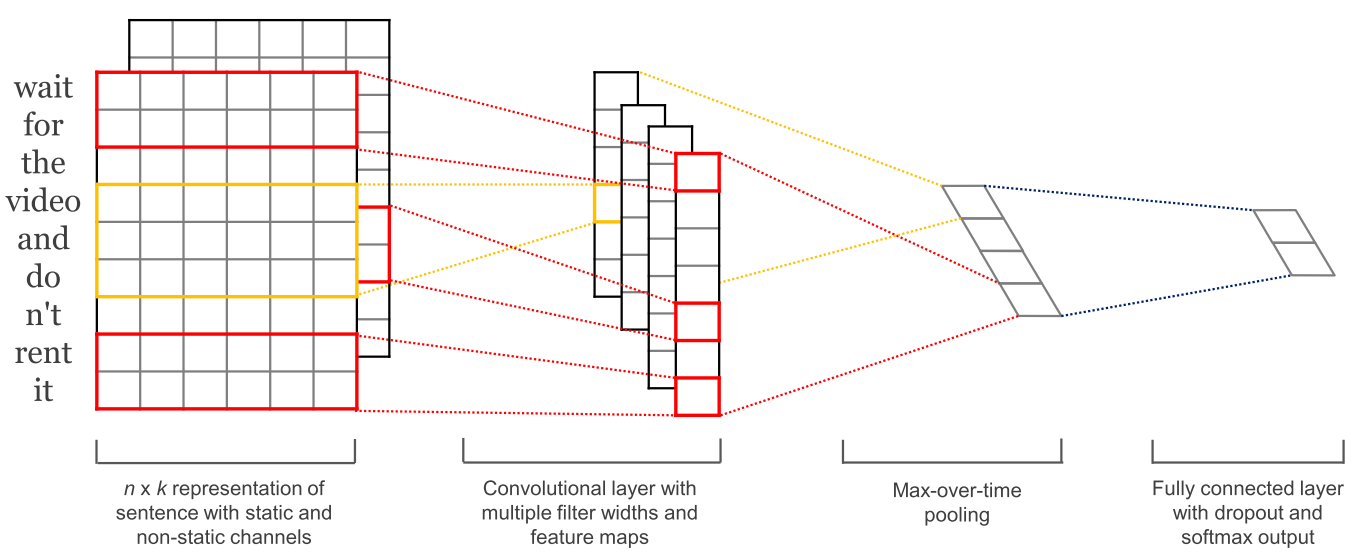
\includegraphics[width=\textwidth]{images/Neuro4-CNN_.png}
  }
  \caption{Пример сверточной нейронной сети}\label{fig:Neuro4-CNN}
\end{figure}

\subsubsection{Рекурсивные нейронные сети}\label{ch:nn:rcnn}
Хотя рекуррентные и сверточные нейросети рассматривают естественный язык как последовательность, по своей сути он иерархичен: слова состоят из фраз и предложений более высокого порядка, которые сами могут быть рекурсивно объединены в соответствии с набором строго определенных правил. Это приводит к идее трактовать предложения как деревья, а не как последовательности. Воплощением данной идеи являются рекурсивные нейронные сети~\cite{socher_2013}. В отличие от рекуррентных сетей, обрабатывающих предложение слева направо или справа налево, рекурсивные сети представляют последовательность снизу вверх или сверху вниз. Новое представление в каждом узле находится при помощи составления представлений дочерних узлов. Пример рекурсивной нейронной сети изображен на рисунке \ref{fig:Neuro5-RNN}.



\begin{figure}[ht]
  \centerfloat{
    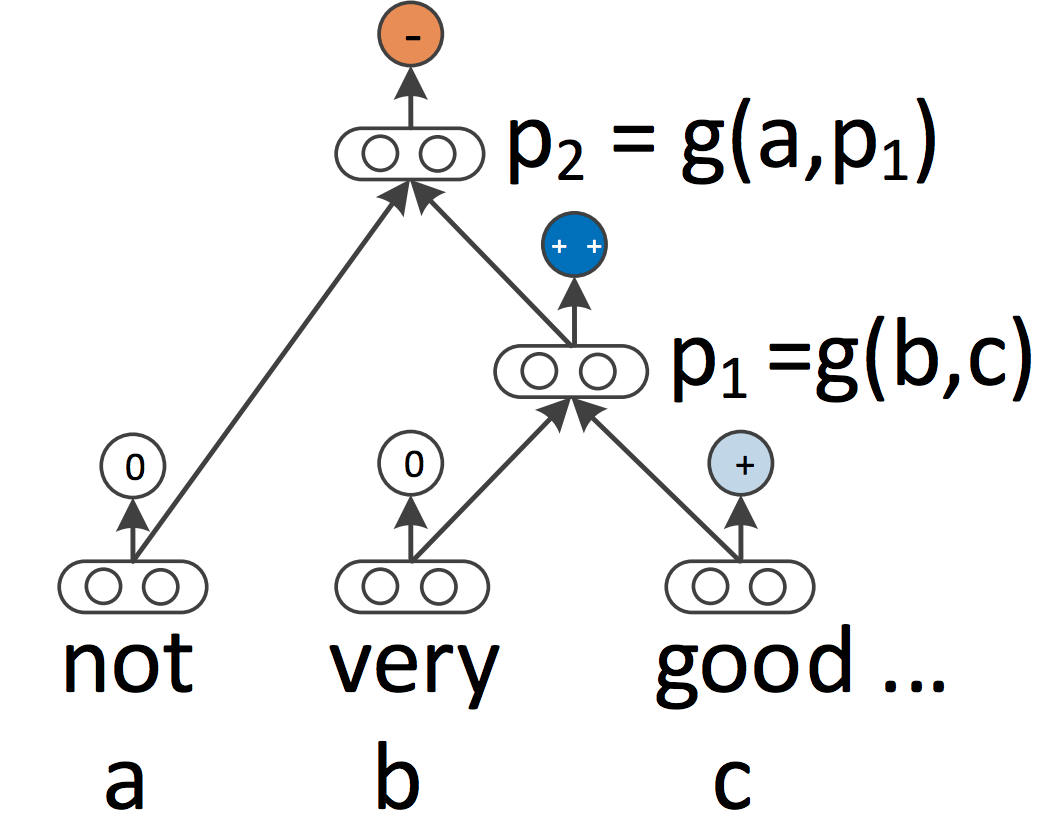
\includegraphics[width=\textwidth]{images/Neuro5-RNN_.png}
  }
  \caption{Пример рекурсивной нейронной сети}\label{fig:Neuro5-RNN}
\end{figure}
\subsection{Нейросети, основанные на памяти}
В середине 2010-х годов стали активно появляться архитектуры нейросетевых моделей, использующие память - скрытые состояния модели, при этом модель сама выбирает, что необходимо извлечь из памяти. 

Из моделей, использующих память, можно выделить сквозные сети памяти \cite{sukhbaatar_2015}, модели с динамической памятью \cite{kumar_2016}, дифференцируемые нейрокомпьютеры \cite{graves_2016}, модели с памятью «ключ-значение» \cite{miller_2016} и пр.
 
Доступ к памяти в таких моделях осуществляется при помощи «схожести» по текущему расстоянию по той или иной метрике, подобным вниманию, и память в модели обычно может записываться и считываться.  Модели отличаются тем, как они реализуют и используют память. Например, сквозные сети памяти обрабатывают ввод несколько раз и только затем обновляют память, чтобы сделать возможным несколько этапов вывода.  Нейронные машины Тьюринга имеют адресацию на основе местоположения, что позволяет им изучать простые компьютерные программы, такие как сортировка.  Модели на основе памяти, как правило, применяются к задачам, где информацию нужно хранить достаточно долго, например, моделирование языка или понимание текста. 